% =====================================================================
%  AetherGrid AI - UML Sequence Diagram (complete project lifecycle)
%  Single page, A3 landscape.  Compile: pdflatex aethergrid_sequence_diagram.tex
% =====================================================================
\documentclass[10pt,a3paper]{article}
\usepackage[T1]{fontenc}
\usepackage[utf8]{inputenc}
\usepackage{helvet}
\renewcommand{\familydefault}{\sfdefault}
\usepackage[landscape,margin=0.8cm]{geometry}
\usepackage{xcolor}
\usepackage{adjustbox}
\usepackage{tikz}
\usetikzlibrary{arrows.meta,calc,backgrounds}
\pagestyle{empty}
\definecolor{ink}{HTML}{1F2A44}
\definecolor{hdrC}{HTML}{DDE9DD}
\definecolor{hdrP}{HTML}{D6E2F3}
\definecolor{hdrA}{HTML}{F3D4D4}
\definecolor{bdP}{HTML}{3B5B88}
\definecolor{bdA}{HTML}{9E2A2B}
\definecolor{actC}{HTML}{E6EFE6}
\definecolor{actP}{HTML}{E4ECF8}
\definecolor{actA}{HTML}{F8E4E4}
\tikzset{
 hc/.style={draw=ink,line width=0.6pt,fill=hdrC,minimum width=2.45cm,minimum height=0.85cm,align=center,font=\fontsize{6.4}{7.4}\selectfont\bfseries,inner sep=2pt},
 hp/.style={hc,draw=bdP,fill=hdrP},
 hh/.style={hc,draw=bdA,fill=hdrA},
 life/.style={draw=ink!45,line width=0.5pt,dash pattern=on 3pt off 2.5pt},
 bC/.style={draw=ink,line width=0.5pt,fill=actC},
 bP/.style={draw=bdP,line width=0.5pt,fill=actP},
 bA/.style={draw=bdA,line width=0.5pt,fill=actA},
 sy/.style={-{Triangle[length=2mm,width=1.6mm]},ink,line width=0.6pt},
 sp/.style={-{Triangle[length=2mm,width=1.6mm]},bdP,line width=0.6pt},
 sa/.style={-{Triangle[length=2mm,width=1.6mm]},bdA,line width=0.6pt},
 rt/.style={-{To[length=2mm,width=2mm]},ink,line width=0.5pt,dash pattern=on 3pt off 2pt},
 rtp/.style={-{To[length=2mm,width=2mm]},bdP,line width=0.5pt,dash pattern=on 3pt off 2pt},
 rta/.style={-{To[length=2mm,width=2mm]},bdA,line width=0.5pt,dash pattern=on 3pt off 2pt},
 ml/.style={font=\fontsize{6}{7}\selectfont,text=ink,fill=white,inner sep=0.8pt},
 mlp/.style={ml,text=bdP},
 mla/.style={ml,text=bdA},
 fr/.style={draw=ink!60,line width=0.6pt,fill=ink!4,fill opacity=0.5},
 ft/.style={draw=ink!60,line width=0.5pt,fill=white,font=\fontsize{6}{7}\selectfont\bfseries,inner xsep=3pt,inner ysep=1.5pt,anchor=north west},
 fg/.style={fill=white,fill opacity=0.9,text opacity=1,font=\fontsize{6}{7}\selectfont\itshape,text=ink,anchor=north west,inner sep=1pt},
}
\begin{document}
\begin{center}
{\Large\bfseries AetherGrid AI \,--\, UML Sequence Diagram}\\[1pt]
{\small End-to-end lifecycle: disruption handling, batch dispatch (Hungarian / GA-VRPTW), agent execution, RL repositioning and invariant verification}
\end{center}
\vspace{-6pt}
\begin{center}
\begin{adjustbox}{max width=\linewidth,max height=\dimexpr\textheight-3.4cm\relax}
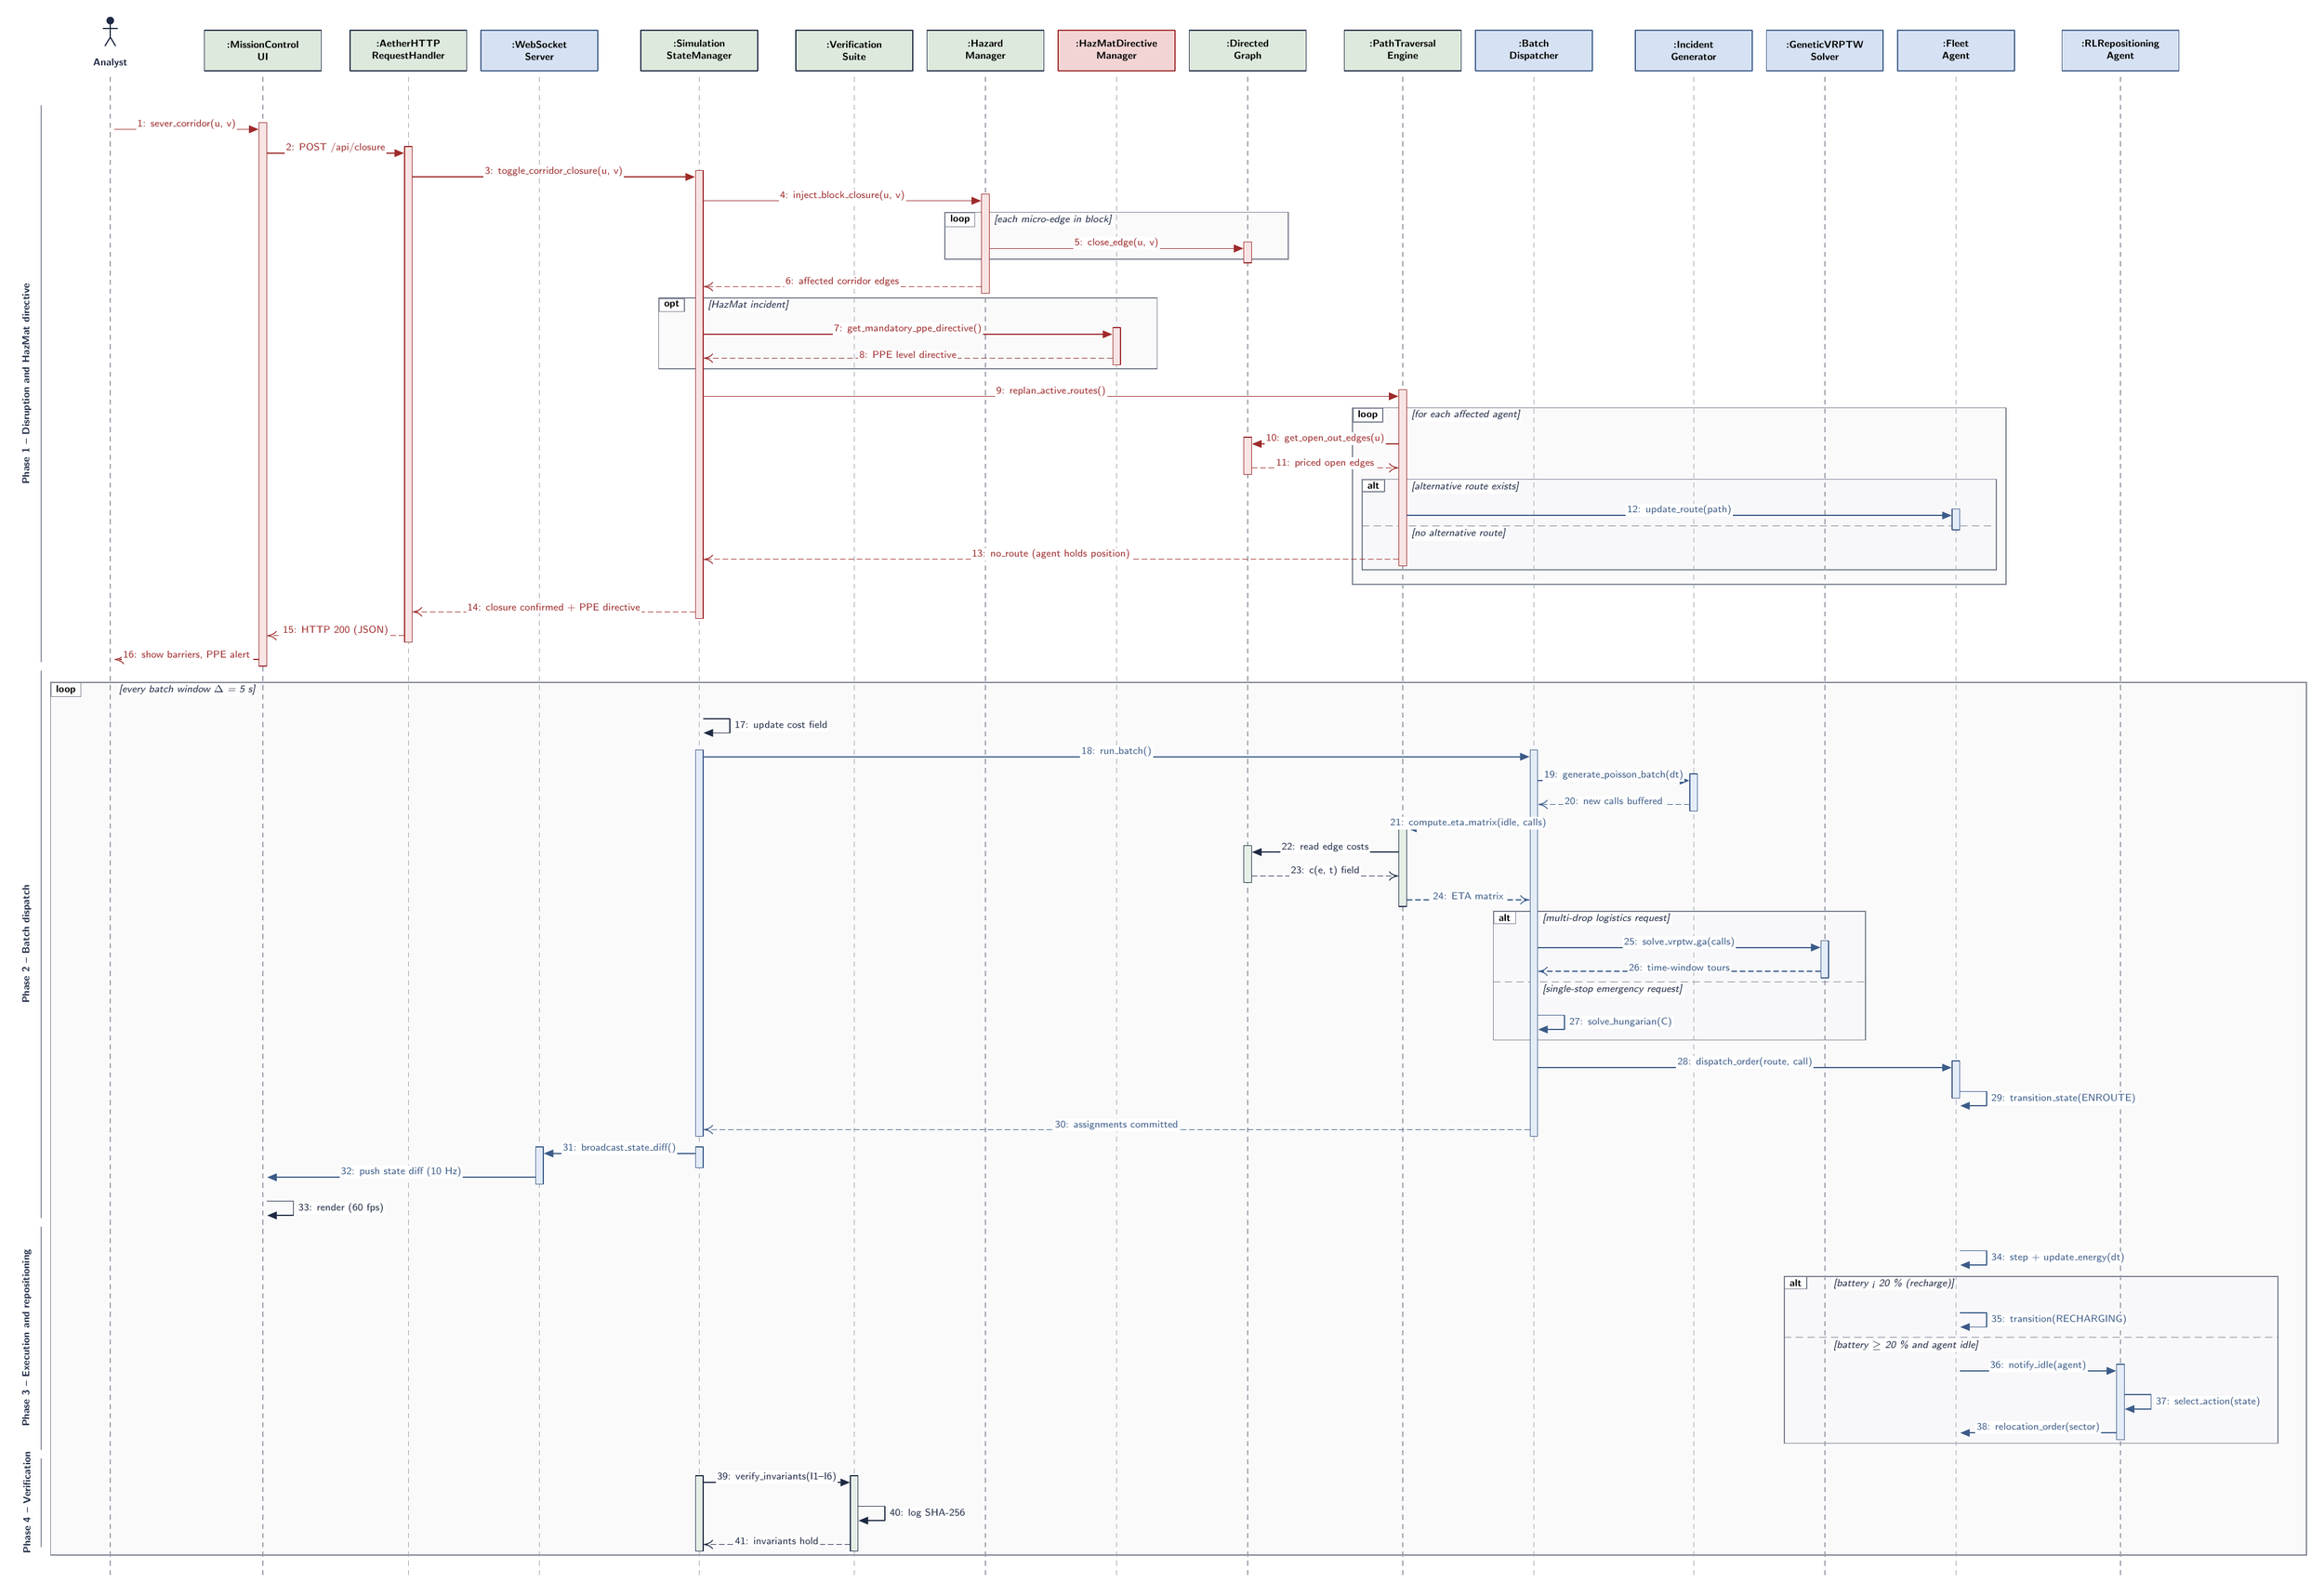
\begin{tikzpicture}[line join=round,line cap=round]

\begin{scope}[on background layer]
\draw[fr] (-1.25,-13.60) rectangle (46.05,-31.90);
\draw[fr] (26.05,-7.84) rectangle (39.75,-11.54);
\draw[fr] (35.10,-26.06) rectangle (45.45,-29.56);
\draw[fr] (29.00,-18.40) rectangle (36.80,-21.10);
\draw[fr] (26.25,-9.34) rectangle (39.55,-11.24);
\draw[fr] (11.50,-5.54) rectangle (21.95,-7.02);
\draw[fr] (17.50,-3.74) rectangle (24.70,-4.72);
\draw[life] (0.00,-0.9) -- (0.00,-32.38);
\draw[life] (3.20,-0.9) -- (3.20,-32.38);
\draw[life] (6.25,-0.9) -- (6.25,-32.38);
\draw[life] (9.00,-0.9) -- (9.00,-32.38);
\draw[life] (12.35,-0.9) -- (12.35,-32.38);
\draw[life] (15.60,-0.9) -- (15.60,-32.38);
\draw[life] (18.35,-0.9) -- (18.35,-32.38);
\draw[life] (21.10,-0.9) -- (21.10,-32.38);
\draw[life] (23.85,-0.9) -- (23.85,-32.38);
\draw[life] (27.10,-0.9) -- (27.10,-32.38);
\draw[life] (29.85,-0.9) -- (29.85,-32.38);
\draw[life] (33.20,-0.9) -- (33.20,-32.38);
\draw[life] (35.95,-0.9) -- (35.95,-32.38);
\draw[life] (38.70,-0.9) -- (38.70,-32.38);
\draw[life] (42.15,-0.9) -- (42.15,-32.38);
\end{scope}
\begin{scope}[shift={(0.00,-0.05)},line width=0.7pt,draw=ink]\fill[ink] (0,0.33) circle (0.08);\draw (0,0.25)--(0,-0.02);\draw (-0.15,0.17)--(0.15,0.17);\draw (0,-0.02)--(-0.11,-0.2);\draw (0,-0.02)--(0.11,-0.2);\end{scope}
\node[font=\fontsize{6.4}{7.4}\selectfont\bfseries,text=ink] at (0.00,-0.62) {Analyst};
\node[hc] at (3.20,-0.35) {:MissionControl\\UI};
\node[hc] at (6.25,-0.35) {:AetherHTTP\\RequestHandler};
\node[hp] at (9.00,-0.35) {:WebSocket\\Server};
\node[hc] at (12.35,-0.35) {:Simulation\\StateManager};
\node[hc] at (15.60,-0.35) {:Verification\\Suite};
\node[hc] at (18.35,-0.35) {:Hazard\\Manager};
\node[hh] at (21.10,-0.35) {:HazMatDirective\\Manager};
\node[hc] at (23.85,-0.35) {:Directed\\Graph};
\node[hc] at (27.10,-0.35) {:PathTraversal\\Engine};
\node[hp] at (29.85,-0.35) {:Batch\\Dispatcher};
\node[hp] at (33.20,-0.35) {:Incident\\Generator};
\node[hp] at (35.95,-0.35) {:GeneticVRPTW\\Solver};
\node[hp] at (38.70,-0.35) {:Fleet\\Agent};
\node[hp] at (42.15,-0.35) {:RLRepositioning\\Agent};
\node[ft] at (17.50,-3.74) {loop};
\node[fg] at (18.49,-3.75) {[each micro-edge in block]};
\node[ft] at (11.50,-5.54) {opt};
\node[fg] at (12.49,-5.55) {[HazMat incident]};
\node[ft] at (26.25,-9.34) {alt};
\node[fg] at (27.24,-9.35) {[alternative route exists]};
\draw[ink!60,dash pattern=on 4pt off 3pt,line width=0.5pt] (26.25,-10.32) -- (39.55,-10.32);
\node[fg] at (27.24,-10.34) {[no alternative route]};
\node[ft] at (26.05,-7.84) {loop};
\node[fg] at (27.24,-7.85) {[for each affected agent]};
\node[ft] at (29.00,-18.40) {alt};
\node[fg] at (29.99,-18.41) {[multi-drop logistics request]};
\draw[ink!60,dash pattern=on 4pt off 3pt,line width=0.5pt] (29.00,-19.88) -- (36.80,-19.88);
\node[fg] at (29.99,-19.90) {[single-stop emergency request]};
\node[ft] at (35.10,-26.06) {alt};
\node[fg] at (36.09,-26.07) {[battery < 20 \% (recharge)]};
\draw[ink!60,dash pattern=on 4pt off 3pt,line width=0.5pt] (35.10,-27.34) -- (45.45,-27.34);
\node[fg] at (36.09,-27.36) {[battery $\geq$ 20 \% and agent idle]};
\node[ft] at (-1.25,-13.60) {loop};
\node[fg] at (0.14,-13.61) {[every batch window $\Delta$ = 5 s]};
\draw[bA] (3.12,-1.86) rectangle (3.28,-13.26);
\draw[bA] (6.17,-2.36) rectangle (6.33,-12.76);
\draw[bA] (12.27,-2.86) rectangle (12.43,-12.26);
\draw[bA] (18.27,-3.36) rectangle (18.43,-5.44);
\draw[bA] (23.77,-4.36) rectangle (23.93,-4.80);
\draw[bA] (21.02,-6.16) rectangle (21.18,-6.94);
\draw[bA] (27.02,-7.46) rectangle (27.18,-11.16);
\draw[bA] (23.77,-8.46) rectangle (23.93,-9.24);
\draw[bP] (38.62,-9.96) rectangle (38.78,-10.40);
\draw[bP] (12.27,-15.02) rectangle (12.43,-23.12);
\draw[bP] (29.77,-15.02) rectangle (29.93,-23.12);
\draw[bP] (33.12,-15.52) rectangle (33.28,-16.30);
\draw[bC] (27.02,-16.52) rectangle (27.18,-18.30);
\draw[bC] (23.77,-17.02) rectangle (23.93,-17.80);
\draw[bP] (35.87,-19.02) rectangle (36.03,-19.80);
\draw[bP] (38.62,-21.54) rectangle (38.78,-22.32);
\draw[bP] (8.92,-23.34) rectangle (9.08,-24.12);
\draw[bP] (12.27,-23.34) rectangle (12.43,-23.78);
\draw[bP] (42.07,-27.90) rectangle (42.23,-29.48);
\draw[bC] (12.27,-30.24) rectangle (12.43,-31.82);
\draw[bC] (15.52,-30.24) rectangle (15.68,-31.82);
\draw[sa] (0.09,-2.00) -- (3.11,-2.00) node[midway,above=-1pt,mla] {1: sever\_corridor(u, v)};
\draw[sa] (3.29,-2.50) -- (6.16,-2.50) node[midway,above=-1pt,mla] {2: POST /api/closure};
\draw[sa] (6.34,-3.00) -- (12.26,-3.00) node[midway,above=-1pt,mla] {3: toggle\_corridor\_closure(u, v)};
\draw[sa] (12.44,-3.50) -- (18.26,-3.50) node[midway,above=-1pt,mla] {4: inject\_block\_closure(u, v)};
\draw[sa] (18.44,-4.50) -- (23.76,-4.50) node[midway,above=-1pt,mla] {5: close\_edge(u, v)};
\draw[rta] (18.26,-5.30) -- (12.44,-5.30) node[midway,above=-1pt,mla] {6: affected corridor edges};
\draw[sa] (12.44,-6.30) -- (21.01,-6.30) node[midway,above=-1pt,mla] {7: get\_mandatory\_ppe\_directive()};
\draw[rta] (21.01,-6.80) -- (12.44,-6.80) node[midway,above=-1pt,mla] {8: PPE level directive};
\draw[sa] (12.44,-7.60) -- (27.01,-7.60) node[midway,above=-1pt,mla] {9: replan\_active\_routes()};
\draw[sa] (27.01,-8.60) -- (23.94,-8.60) node[midway,above=-1pt,mla] {10: get\_open\_out\_edges(u)};
\draw[rta] (23.94,-9.10) -- (27.01,-9.10) node[midway,above=-1pt,mla] {11: priced open edges};
\draw[sp] (27.19,-10.10) -- (38.61,-10.10) node[midway,above=-1pt,mlp] {12: update\_route(path)};
\draw[rta] (27.01,-11.02) -- (12.44,-11.02) node[midway,above=-1pt,mla] {13: no\_route (agent holds position)};
\draw[rta] (12.26,-12.12) -- (6.34,-12.12) node[midway,above=-1pt,mla] {14: closure confirmed + PPE directive};
\draw[rta] (6.16,-12.62) -- (3.29,-12.62) node[midway,above=-1pt,mla] {15: HTTP 200 (JSON)};
\draw[rta] (3.11,-13.12) -- (0.09,-13.12) node[midway,above=-1pt,mla] {16: show barriers, PPE alert};
\draw[sy] (12.44,-14.36) -- (12.99,-14.36) -- (12.99,-14.66) -- (12.44,-14.66);
\node[ml,anchor=west] at (13.06,-14.51) {17: update cost field};
\draw[sp] (12.44,-15.16) -- (29.76,-15.16) node[midway,above=-1pt,mlp] {18: run\_batch()};
\draw[sp] (29.94,-15.66) -- (33.11,-15.66) node[midway,above=-1pt,mlp] {19: generate\_poisson\_batch(dt)};
\draw[rtp] (33.11,-16.16) -- (29.94,-16.16) node[midway,above=-1pt,mlp] {20: new calls buffered};
\draw[sp] (29.76,-16.66) -- (27.19,-16.66) node[midway,above=-1pt,mlp] {21: compute\_eta\_matrix(idle, calls)};
\draw[sy] (27.01,-17.16) -- (23.94,-17.16) node[midway,above=-1pt,ml] {22: read edge costs};
\draw[rt] (23.94,-17.66) -- (27.01,-17.66) node[midway,above=-1pt,ml] {23: c(e, t) field};
\draw[rtp] (27.19,-18.16) -- (29.76,-18.16) node[midway,above=-1pt,mlp] {24: ETA matrix};
\draw[sp] (29.94,-19.16) -- (35.86,-19.16) node[midway,above=-1pt,mlp] {25: solve\_vrptw\_ga(calls)};
\draw[rtp] (35.86,-19.66) -- (29.94,-19.66) node[midway,above=-1pt,mlp] {26: time-window tours};
\draw[sp] (29.94,-20.58) -- (30.49,-20.58) -- (30.49,-20.88) -- (29.94,-20.88);
\node[mlp,anchor=west] at (30.56,-20.73) {27: solve\_hungarian(C)};
\draw[sp] (29.94,-21.68) -- (38.61,-21.68) node[midway,above=-1pt,mlp] {28: dispatch\_order(route, call)};
\draw[sp] (38.79,-22.18) -- (39.34,-22.18) -- (39.34,-22.48) -- (38.79,-22.48);
\node[mlp,anchor=west] at (39.41,-22.33) {29: transition\_state(ENROUTE)};
\draw[rtp] (29.76,-22.98) -- (12.44,-22.98) node[midway,above=-1pt,mlp] {30: assignments committed};
\draw[sp] (12.26,-23.48) -- (9.09,-23.48) node[midway,above=-1pt,mlp] {31: broadcast\_state\_diff()};
\draw[sp] (8.91,-23.98) -- (3.29,-23.98) node[midway,above=-1pt,mlp] {32: push state diff (10 Hz)};
\draw[sy] (3.29,-24.48) -- (3.84,-24.48) -- (3.84,-24.78) -- (3.29,-24.78);
\node[ml,anchor=west] at (3.91,-24.63) {33: render (60 fps)};
\draw[sp] (38.79,-25.52) -- (39.34,-25.52) -- (39.34,-25.82) -- (38.79,-25.82);
\node[mlp,anchor=west] at (39.41,-25.67) {34: step + update\_energy(dt)};
\draw[sp] (38.79,-26.82) -- (39.34,-26.82) -- (39.34,-27.12) -- (38.79,-27.12);
\node[mlp,anchor=west] at (39.41,-26.97) {35: transition(RECHARGING)};
\draw[sp] (38.79,-28.04) -- (42.06,-28.04) node[midway,above=-1pt,mlp] {36: notify\_idle(agent)};
\draw[sp] (42.24,-28.54) -- (42.79,-28.54) -- (42.79,-28.84) -- (42.24,-28.84);
\node[mlp,anchor=west] at (42.86,-28.69) {37: select\_action(state)};
\draw[sp] (42.06,-29.34) -- (38.79,-29.34) node[midway,above=-1pt,mlp] {38: relocation\_order(sector)};
\draw[sy] (12.44,-30.38) -- (15.51,-30.38) node[midway,above=-1pt,ml] {39: verify\_invariants(I1--I6)};
\draw[sy] (15.69,-30.88) -- (16.24,-30.88) -- (16.24,-31.18) -- (15.69,-31.18);
\node[ml,anchor=west] at (16.31,-31.03) {40: log SHA-256};
\draw[rt] (15.51,-31.68) -- (12.44,-31.68) node[midway,above=-1pt,ml] {41: invariants hold};
\node[rotate=90,font=\fontsize{6.2}{7.2}\selectfont\bfseries,text=ink] at (-1.75,-7.34) {Phase 1 -- Disruption and HazMat directive};
\draw[ink!50,line width=0.5pt] (-1.45,-1.50) -- (-1.45,-13.17);
\node[rotate=90,font=\fontsize{6.2}{7.2}\selectfont\bfseries,text=ink] at (-1.75,-19.09) {Phase 2 -- Batch dispatch};
\draw[ink!50,line width=0.5pt] (-1.45,-13.36) -- (-1.45,-24.83);
\node[rotate=90,font=\fontsize{6.2}{7.2}\selectfont\bfseries,text=ink] at (-1.75,-27.35) {Phase 3 -- Execution and repositioning};
\draw[ink!50,line width=0.5pt] (-1.45,-25.02) -- (-1.45,-29.69);
\node[rotate=90,font=\fontsize{6.2}{7.2}\selectfont\bfseries,text=ink] at (-1.75,-30.80) {Phase 4 -- Verification};
\draw[ink!50,line width=0.5pt] (-1.45,-29.88) -- (-1.45,-31.73);
\end{tikzpicture}
\end{adjustbox}
\end{center}
\vspace{4pt}
\begin{center}

\begin{tikzpicture}[font=\footnotesize]
 \draw[sy] (0,0)--(1,0); \node[anchor=west,text=ink] at (1.1,0) {Synchronous call};
 \draw[rt] (4.3,0)--(5.3,0); \node[anchor=west,text=ink] at (5.4,0) {Return};
 \draw[sa] (7.3,0)--(8.3,0); \node[anchor=west,text=bdA] at (8.4,0) {Disruption / HazMat};
 \draw[sp] (12.4,0)--(13.4,0); \node[anchor=west,text=bdP] at (13.5,0) {Planned subsystem};
 \draw[bC] (17.2,-0.15) rectangle (17.5,0.15); \node[anchor=west,text=ink] at (17.6,0) {Activation};
 \node[hc,minimum width=0.9cm,minimum height=0.35cm] at (20.3,0) {}; \node[anchor=west,text=ink] at (20.9,0) {Implemented};
 \node[hp,minimum width=0.9cm,minimum height=0.35cm] at (23.8,0) {}; \node[anchor=west,text=ink] at (24.4,0) {Planned};
 \node[hh,minimum width=0.9cm,minimum height=0.35cm] at (26.9,0) {}; \node[anchor=west,text=ink] at (27.5,0) {HazMat safety};
\end{tikzpicture}
\end{center}
\end{document}
